\documentclass[tikz]{standalone}
\usepackage[sfdefault,light]{roboto}
\usetikzlibrary{shapes, arrows, positioning, fit, backgrounds}
\tikzset{every picture/.style={/utils/exec={\sffamily}}}
\definecolor{MyGreen}{HTML}{41B3A3}
\begin{document}
    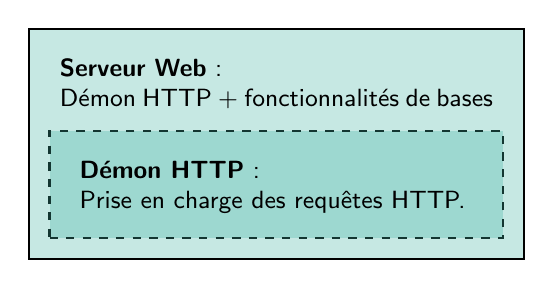
\begin{tikzpicture}[
			every node/.style={draw,rectangle,thick, font=\small},
			env/.style={draw,rectangle,thick,inner sep=0.25cm}
		]
			\node (http) [anchor=south west,draw=none] at (0,0) 
			{
                \begin{minipage}[t][.6cm]{5cm}
                    \textbf{Démon HTTP} : \\
                    Prise en charge des requêtes HTTP.
				\end{minipage}
            };
			\node (web) [above=0.4cm of http,draw=none] 
			{
                \begin{minipage}[t]{5.5cm}
                    \textbf{Serveur Web} :\\
                    Démon HTTP + fonctionnalités de bases
				\end{minipage}
};
			
			\begin{scope}[on background layer]
				\node (envHttp) [env,fit=(http),fill opacity=0.3,fill=MyGreen,dashed] {};
				\node (envWeb) [env,fit=(web) (envHttp),fill opacity=0.3,fill=MyGreen] {};
			\end{scope}
		\end{tikzpicture}
\end{document}